\section{Stress Detection}
From a user's input sentence $c$, \emph{TeenChat} firstly tries to sense whether the user has some stress or not
based on our stress-related emotion lexicon in Table 1.
Meanwhile, it builds a linguistic dependency tree for $c$, whose root node is the core
word of the sentence.
\emph{TeenChat} analyzes all possible linkage between the stress emotion word and stress category/sub-category words in the tree,
and returns a set of triples of the form:
\texttt{(Stress, Category:$l_c$, SubCategory:$l_s$)},
where \texttt{Stress} takes value 0 (meaning no stress detected) or 1 (meaning stress detected),
$l_c$ is the path length between the negative emotional word and the category node,
and $l_s$ is the path length between the negative emotional word and the sub-category node.
$l_c$/$l_s$ can be null if there exists no path linking the negative emotion word and
the category/sub-category word.
\begin{table}
\label{tab:lexicons}
\begin{minipage}{\textwidth}
\centering
\caption{Stress-Related Lexicons}

\begin{tabular}{ll|l} \\ \hline
\multicolumn{3}{l}{\textbf{I. Stress Emotion Lexicon}} \\ \hline
\multicolumn{2}{l|}{Negative Emotion} & \emph{stress, stressful, pressure,  nervous, unhappy, annoyed,} \\
  &      & \emph{annoying, bad, sad, etc.} \\ \hline
\multicolumn{2}{l|}{Positive Emotion} & \emph{happy, relaxed, good, fun, etc.} \\ \hline
\multicolumn{2}{l|}{Negation}  & \emph{no, not, neither, etc.} \\ \hline

\multicolumn{3}{l}{\textbf{II. Stress Category/Sub-Category Lexicon}} \\ \hline
STUDY & Homework & \emph{homework, project, practice, assignment, etc.} \\ \cline{2-3}
      & Exam     & \emph{exam, grade, mark, rank, score, etc.} \\ \cline{2-3}
      & General  & \emph{history, math, physical, etc.}  \\ \hline
SELF-      & Appearance & \emph{ugly, fat, stout, etc.} \\ \cline{2-3}
COGNITION      & Health     & \emph{sleepless, flustered, insomnia, fracture, stomachache, etc.} \\ \cline{2-3}
& Inner-feeling & \emph{foolish, stupid, awkward, incapable, self-distrust, etc.} \\ \cline{2-3}
               & General & \emph{unconfident, inferior, abased, weak, etc.} \\ \hline
INTER- & Family & \emph{father, mother, brother, sister, uncle, aunt, etc.} \\\cline{2-3}
PERSONAL & Teacher & \emph{teacher, school, regulation, schoolmaster, etc.} \\ \cline{2-3}
& Friend & \emph{classmate, friendship, etc.} \\ \cline{2-3}
& General & \emph{quarrel, criticize, ridicule, etc.} \\ \hline
AFFECTION & Lover  &  \emph{boyfriend, girlfriend etc.}  \\ \cline{2-3}
  & Partner    &  \emph{partner, etc.}    \\ \cline{2-3}
& General & \emph{break-up, separate, secret-love, unrequited love, etc.} \\ \hline
GENERAL & \multicolumn{2}{l}{(unknown category and sub-category)}   \\ \hline
\end{tabular}
\end{minipage}
\end{table}

\begin{example}
Take sentence ``\emph{Always quarrelling with friends at school, so annoyed!}"  for example.
Fig.~\ref{fig:dependenceTree} gives its linguistic dependency tree, constructed by the
linguistic analysis tool LTP~\cite{Che10}.
The stress-related negative emotion word ``\emph{annoyed}" is linked to
``\emph{quarrel}" via a 1-length path, and to
``\emph{friend}" via a 3-length path.
As ``\emph{quarrel}" belongs to stress category INTER-PERSONAL,
and ``\emph{friend}" to its sub-category Friend, a user's stress in INTER-PERSONAL,
in particular in the Friend aspect, is sensed from the sentence, denoted
as \texttt{(1, INTER-PERSONAL:1, Friend:3)}.
%\boxend
\end{example}

In case multiple stress categories/sub-categories are sensed,
the one with the shortest path between the negative emotion word and
the stress category or sub-category word is considered as the primary stress category/sub-category.
When the path length cannot help make distinction, the category similar to the
historic stress category will be taken as the primary one.
If the above also fails, the primary one is randomly determined.
In this way, from each user's input sentence $c$, a detection result
\texttt{(c.Stress, c.Category, c.SubCategory)} is returned, where
\texttt{c.Stress=0} indicates no stress is discovered from the current sentence $c$, and
\texttt{c.Category/c.SubCategory=null} indicates no category/sub-category word is found in $c$.

Considering user's short dialogue inputs, as well as the consecutiveness of stressful emotion remaining
during conversation, we keep and refresh user's historic stress status,
(\texttt{(h.Stress, h.Category, h.SubCategory)}) detected from the previous sentences as follows. \\
\noindent (1) When no stress is detected from the current sentence $c$, but detected from the history,
if \texttt{h.Category==c.Category} and
\texttt{h.SubCategory==c.SubCategory},\\we mark \texttt{c.Stress=1}. \\
\noindent (2) When stress is detected from the current sentence $c$ with a concrete category/
sub-category, which
is/are missing from the history, we assign \\
\texttt{h.Category=c.Category} and \texttt{h.SubCategory=c.SubCategory}.
\begin{figure}
\makeatletter\def\@captype{figure}\makeatother
\begin{minipage}{.51\textwidth}
\centering
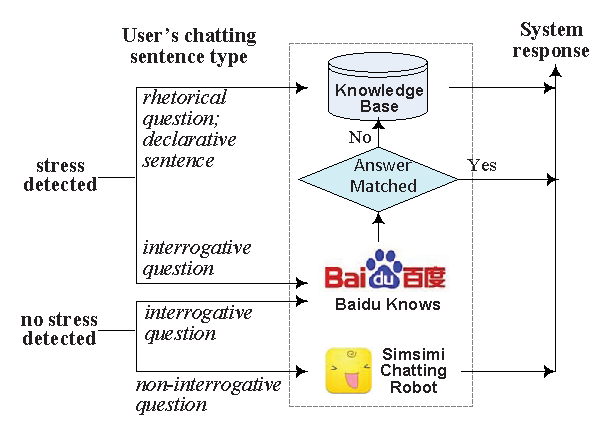
\includegraphics[height=3.5cm]{figs/ResponseStrategy.eps}
\caption{\emph{TeenChat} response strategies}
\label{fig:ResponseStrategy}
\end{minipage}
\makeatletter\def\@captype{figure}\makeatother
\begin{minipage}{.45\textwidth}
\centering
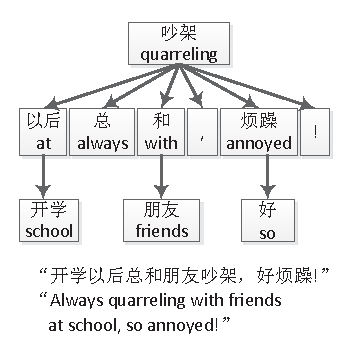
\includegraphics[height=3.5cm]{figs/dependenceTreeExample.eps}
\caption{A dependence tree example}
\label{fig:dependenceTree}
\end{minipage}
\end{figure}
